\documentclass[10pt, 169]{beamer}

\usepackage{polyglossia}
\usepackage{csquotes}
\usepackage{bm}
\usepackage{datetime}
\usepackage{fontspec}
\usepackage{microtype}
\usepackage{color}
\usepackage{url}
\usepackage{pgfplots}
\usepackage{hyperref}
\usepackage{amsfonts}
\usepackage{amsmath}
\usepackage{amsthm}
\usepackage{subcaption}
\usepackage[backend=biber,style=iso-authoryear,sortlocale=en_US,autolang=other,bibencoding=UTF8]{biblatex}
\usepackage{booktabs}
\usepackage{graphics}
\usepackage{pifont}
\usepackage{ulem}
\usepackage{tikz}

\usepgfplotslibrary{fillbetween}
\usetikzlibrary{arrows,automata,shapes,calc, patterns, backgrounds}

\addbibresource{zotero.bib}

\setdefaultlanguage{english}
\setmainfont{TeX Gyre Termes}
\usetheme{Boadilla}
\usecolortheme{crane}
\setbeamertemplate{title page}[default][rounded=true,shadow=false]
\setbeamertemplate{section in toc}[ball unnumbered]
\setbeamertemplate{bibliography item}{}

\hypersetup{
	pdfencoding=auto,
	unicode=true,
	citecolor=green,
	filecolor=blue,
	linkcolor=red,
	urlcolor=blue
}

\makeatletter
\newcommand*{\currentSection}{\@currentlabelname}
\makeatother

\newcommand{\mathmat}{\ensuremath{\mathbf}}

\title[DDny 2023]
{
	Which Graph Properties Affect GNN Performance for a Given Downstream Task?
}

\newdate{presentation}{10}{11}{2023}
\date[November 2023]{Doktorandské dny KM FJFI, \displaydate{presentation}}

\author[Procházka et al.]{
	Pavel Procházka\inst{1} \and
	Michal Mareš\inst{1,2} \and
	\underline{Marek Dědič}\inst{1,2}
}
\institute[Cisco \& CTU]{
	\inst{1}Cisco Systems, Inc. \and
	\inst{2}Czech Technical University in Prague
}

% Title card
\AtBeginSection[]{
	\begin{frame}
	\vfill
	\centering
	\begin{beamercolorbox}[sep = 8pt,center,shadow = true,rounded = true]{title}
		\usebeamerfont{title}\insertsectionhead\par%
	\end{beamercolorbox}
	\vfill
\end{frame}
}

\begin{document}

\begin{frame}
	\titlepage
\end{frame}


\begin{frame}
	\frametitle{Motivation -- Representation by Graph}
	{\scalebox{0.45}{\newcommand\user[2]{
	\begin{scope}[xshift=#1cm, yshift=#2cm]
		\clip (0, 0) circle (0.5);
		\fill[black] (0, 0) circle (0.5);
		\fill[white] (0, 0) circle (0.48);
		\fill[black] (0, -0.675) circle (0.4);
		\fill[black] (0, 0.075) circle (0.24);
	\end{scope}
}

\newcommand\ip[2]{
	\begin{scope}[xshift=#1cm, yshift=#2cm]
		%\rectangle[fill=black, rounded corners=0.2cm] (-0.5, -0.7) -- (0.5, 0.7);
		\draw[fill=black, thick, rounded corners=0.15cm] (-0.3, -0.5) rectangle (0.3, 0.5);
		\draw[fill=white] (0, -0.3) circle (0.1);
		\draw[fill=white, rounded corners=0.07cm] (-0.2, -0.1) rectangle (0.2, 0.0);
		\draw[fill=white, rounded corners=0.07cm] (-0.2, 0.1) rectangle (0.2, 0.2);
		\draw[fill=white, rounded corners=0.07cm] (-0.2, 0.3) rectangle (0.2, 0.4);
	\end{scope}
}

\newcommand\www[2]{
	\begin{scope}[xshift=#1cm, yshift=#2cm]
		\clip (0, 0) circle (0.5);
		\fill[yellow!65!black] (0, 0) circle (0.5);
		\fill[white] (-0.5, -0.175) rectangle (0.5,0.175);
		\node[text=yellow!65!black] at (0,0) {www};
	\end{scope}
}

\newcommand\malwww[2]{
	\begin{scope}[xshift=#1cm, yshift=#2cm]
		\clip (0, 0) circle (0.5);
		\fill[red!65!black] (0, 0) circle (0.5);
		\fill[white] (-0.5, -0.175) rectangle (0.5,0.175);
		\node[text=yellow!65!black] at (0,0) {www};
	\end{scope}
}

\newcommand\wwwline[3]{
	\node[circle, minimum size=1.1cm] (#3) at (0, #1) {};
	\www{0}{#1}
	\node[text width=50mm, align=right] at (-5, #1) {#2};
}

\newcommand\malwwwline[3]{
	\node[circle, minimum size=1.1cm] (#3) at (0, #1) {};
	\malwww{0}{#1}
	\node[text width=50mm, align=right] at (-5, #1) {#2};
}

\newcommand\userline[2]{
	\node[circle, minimum size=1.1cm] (#2) at (5, #1) {};
	\user{5}{#1}
	\node[text width=50mm, align=left] at (10, #1) {#2};
}

\newcommand\ipline[3]{
	\node[circle, minimum size=1.1cm] (#3) at (5, #1) {};
	\ip{5}{#1}
	\node[text width=50mm, align=left] at (10, #1) {#2};
}


\begin{tikzpicture}

\node at (-15, 4) (x)
{
\begin{tabular}{|c|c|c|c|}
\hline
$\bm{time}$ & $\bm{user}$ & $\bm{domain}$ & $\bm{ip}$ \\
\hline
$t_1$&alice& candidate.com& 1.12.2.3\\
$t_2$&bob& somedomain.ch& 2.7.12.1\\
$t_3$&bob& ransomware.com& 2.7.12.1\\
$t_4$&david& unknown.com & 1.12.2.3\\
$t_5$&bob& evil.com & 1.12.2.3 \\
$t_6$&charlie& candidate.com & 1.12.2.3 \\
$t_7$&bob & somedomain.ch& 2.7.12.1 \\
$t_8$&david& unknown.com & 1.12.2.3\\
\vdots &\vdots &\vdots &\vdots \\
\hline
\end{tabular}
};

%{
%$\left\{\begin{array}{c}
%alice, candidate.com, 1.12.2.3\\
%bob, somedomain.ch, 2.7.12.1\\
%bob, ransomware.com, 2.7.12.1\\
%david, unknown.com , 1.12.2.3\\
%bob, evil.com , 1.12.2.3 \\
%charlie, candidate.com , 1.12.2.3 \\
%bob, somedomain.ch, 2.7.12.1 \\
%\dots
%\end{array}\right\}$};
%}
\begin{scope}[scale=0.7, yshift=4.5cm]   
  \malwwwline{-2}{evil.com}{D1};
  \malwwwline{-0.5}{ransomware.com}{D2};
  \wwwline{4}{candidate.com}{D5};
  \ipline{-1}{1.12.2.3}{i1}
  \userline{4.2}{Alice};
  \draw (Alice) -- (D1);
  \draw (Alice) -- (D2);
  \draw (i1) -- (D1);
  \draw (Alice) -- (D5);
  \draw (i1) -- (D5);
  \wwwline{1}{unknown.com}{D3};
  \wwwline{2.5}{somedomain.ch}{D4};
  \ipline{-2.2}{2.7.12.1}{i2}
  \userline{0.6}{David};
  \userline{1.8}{Charlie};
  \userline{3}{Bob};
  \draw (Alice) -- (D3);
  \draw (Bob) -- (D1);
  \draw (Bob) -- (D2);
  \draw (Bob) -- (D1);
  \draw (David) -- (D1);
  \draw (i2) -- (D2);
  \draw (Bob) -- (D4);
  \draw (David) -- (D3);
  \draw (Charlie) -- (D4);
  \draw (Charlie) -- (D5);
  \draw (i1) -- (D3);
  \draw (i2) -- (D4);

\end{scope}


\begin{scope}[scale=0.7, yshift=-4.5cm]  
\node[circle, minimum size=1.1cm] (d1) at (-2, 3) {};
\malwww{-2}{3}	\node[text width=50mm, align=right] at (-6.5, 3) {evil.com};

\node[circle, minimum size=1.1cm] (d2) at (2, 3) {};
\malwww{2}{3}	\node[text width=50mm, align=right] at (3.5, 3) {ransomware.com};

\node[circle, minimum size=1.1cm] (d3) at (-3, 0) {};
\www{-3}{0}	\node[text width=50mm, align=right] at (-7.5, 0) {somedomain.ch};

\node[circle, minimum size=1.1cm] (d4) at (3, 0.5) {};
\www{3}{0.5}	\node[text width=50mm, align=right] at (4, 0.5) {unknown.com};

\node[circle, minimum size=1.1cm] (d5) at (0.5, -2) {};
\www{0.5}{-2}	\node[text width=50mm, align=right] at (-3.8, -2) {candidate.com};

\draw (d1) -- (d2);
\draw (d1) -- (d3);
\draw (d1) -- (d4);
\draw (d2) -- (d3);
\draw (d2) -- (d5);
\draw (d3) -- (d5);
\draw (d4) -- (d5);

\end{scope}

\uncover<2>{
\node[font=\huge, text width=110mm, align=left] at (-13, -2) {
\alert{How to choose the best graph?}
};
}


\uncover<3->{
    \node[font=\huge, text width=110mm, align=left] at (-13, -2) {
How to choose the best graph?
};
    \node [font=\LARGE, text width=110mm, align=left] (top)    at (-13,-3.5) {$\bullet$ Performance on a given task};
    \node [font=\LARGE, text width=110mm, align=left] (middle) at (-13,-4.5)  {$\bullet$ Efficient data representation};
    \node [font=\LARGE, text width=110mm, align=left] (bottom) at (-13,-5.5)  {$\bullet$ Interpretation of edges};
}

\end{tikzpicture}
}} 
\end{frame}

\begin{frame}
	\frametitle{Graph Composition -- Naive Approach}
	{\scalebox{0.45}{\newcommand\user[2]{
	\begin{scope}[xshift=#1cm, yshift=#2cm]
		\clip (0, 0) circle (0.5);
		\fill[black] (0, 0) circle (0.5);
		\fill[white] (0, 0) circle (0.48);
		\fill[black] (0, -0.675) circle (0.4);
		\fill[black] (0, 0.075) circle (0.24);
	\end{scope}
}

\newcommand\ip[2]{
	\begin{scope}[xshift=#1cm, yshift=#2cm]
		%\rectangle[fill=black, rounded corners=0.2cm] (-0.5, -0.7) -- (0.5, 0.7);
		\draw[fill=black, thick, rounded corners=0.15cm] (-0.3, -0.5) rectangle (0.3, 0.5);
		\draw[fill=white] (0, -0.3) circle (0.1);
		\draw[fill=white, rounded corners=0.07cm] (-0.2, -0.1) rectangle (0.2, 0.0);
		\draw[fill=white, rounded corners=0.07cm] (-0.2, 0.1) rectangle (0.2, 0.2);
		\draw[fill=white, rounded corners=0.07cm] (-0.2, 0.3) rectangle (0.2, 0.4);
	\end{scope}
}

\newcommand\www[2]{
	\begin{scope}[xshift=#1cm, yshift=#2cm]
		\clip (0, 0) circle (0.5);
		\fill[yellow!65!black] (0, 0) circle (0.5);
		\fill[white] (-0.5, -0.175) rectangle (0.5,0.175);
		\node[text=yellow!65!black] at (0,0) {www};
	\end{scope}
}

\newcommand\malwww[2]{
	\begin{scope}[xshift=#1cm, yshift=#2cm]
		\clip (0, 0) circle (0.5);
		\fill[red!65!black] (0, 0) circle (0.5);
		\fill[white] (-0.5, -0.175) rectangle (0.5,0.175);
		\node[text=yellow!65!black] at (0,0) {www};
	\end{scope}
}

\newcommand\wwwline[3]{
	\node[circle, minimum size=1.1cm] (#3) at (0, #1) {};
	\www{0}{#1}
	\node[text width=50mm, align=right] at (-5, #1) {#2};
}

\newcommand\malwwwline[3]{
	\node[circle, minimum size=1.1cm] (#3) at (0, #1) {};
	\malwww{0}{#1}
	\node[text width=50mm, align=right] at (-5, #1) {#2};
}

\newcommand\userline[2]{
	\node[circle, minimum size=1.1cm] (#2) at (5, #1) {};
	\user{5}{#1}
	\node[text width=50mm, align=left] at (10, #1) {#2};
}

\newcommand\ipline[3]{
	\node[circle, minimum size=1.1cm] (#3) at (5, #1) {};
	\ip{5}{#1}
	\node[text width=50mm, align=left] at (10, #1) {#2};
}


\begin{tikzpicture}

\node at (-15, 4) (x)
{
\begin{tabular}{cccc}
    \toprule
    $\bm{time}$ & $\bm{user}$ & $\bm{domain}$ & $\bm{ip}$ \\
    \midrule
    $t_1$&alice& candidate.com& 1.12.2.3\\
    $t_2$&bob& somedomain.ch& 2.7.12.1\\
    $t_3$&bob& ransomware.com& 2.7.12.1\\
    $t_4$&david& unknown.com & 1.12.2.3\\
    $t_5$&bob& evil.com & 1.12.2.3 \\
    $t_6$&charlie& candidate.com & 1.12.2.3 \\
    $t_7$&bob & somedomain.ch& 2.7.12.1 \\
    $t_8$&david& unknown.com & 1.12.2.3\\
    \vdots &\vdots &\vdots &\vdots \\
    \bottomrule
\end{tabular}
};

\begin{scope}[scale=0.6, xshift=-8cm, yshift=9cm]  
\node[circle, minimum size=1.1cm] (d1) at (-2, 3) {};
\malwww{-2}{3}	
\node[circle, minimum size=1.1cm] (d2) at (2, 3) {};
\malwww{2}{3}	
\node[circle, minimum size=1.1cm] (d3) at (-3, 0) {};
\www{-3}{0}
\node[circle, minimum size=1.1cm] (d4) at (3, 0.5) {};
\www{3}{0.5}	
\node[circle, minimum size=1.1cm] (d5) at (0.5, -2) {};
\www{0.5}{-2}
\draw (d1) -- (d2);
\draw (d1) -- (d3);
\draw (d1) -- (d4);
\draw (d2) -- (d3);
\draw (d2) -- (d5);
\draw (d3) -- (d5);
\draw (d4) -- (d5);
\end{scope}

\begin{scope}[scale=0.6, xshift=-8cm, yshift=2cm]  
\node[circle, minimum size=1.1cm] (d11) at (-2, 3) {};
\malwww{-2}{3}	
\node[circle, minimum size=1.1cm] (d22) at (2, 3) {};
\malwww{2}{3}	
\node[circle, minimum size=1.1cm] (d33) at (-3, 0) {};
\www{-3}{0}
\node[circle, minimum size=1.1cm] (d44) at (3, 0.5) {};
\www{3}{0.5}	
\node[circle, minimum size=1.1cm] (d55) at (0.5, -2) {};
\www{0.5}{-2}
\draw (d11) -- (d22);
\draw (d11) -- (d44);
\draw (d22) -- (d33);
\draw (d22) -- (d55);
\draw (d33) -- (d55);
\end{scope}

\begin{scope}[scale=0.6,  xshift=-8cm, yshift=-6cm]   
  \malwww{-2}{-2} \node[minimum size=0.8cm] at (-2, -2) (D1) {};
  \malwww{-2}{-0.5}  \node[minimum size=0.8cm] at (-2, -0.5) (D2) {};
  \www{-2}{4} \node[minimum size=0.8cm] at (-2, 4) (D5) {};
  \ip{2}{-1} \node[minimum size=0.8cm] at (2, -1) (i1) {};
  \user{2}{4.2} \node[minimum size=0.8cm] at (2, 4.2)(Alice) {};
  \draw (Alice) -- (D1);
  \draw (Alice) -- (D2);
  \draw (i1) -- (D1);
  \draw (Alice) -- (D5);
  \draw (i1) -- (D5);
  \www{-2}{1}  \node[minimum size=0.8cm] at (-2, 1) (D3) {};
  \www{-2}{2.5}  \node[minimum size=0.8cm] at (-2, 2.5) (D4) {};
  \ip{2}{-2.2}  \node[minimum size=0.8cm] at (2, 2) (i2) {};
  \user{2}{0.6}  \node[minimum size=0.8cm] at (2, 0.6) (David) {};
  \user{2}{1.8}  \node[minimum size=0.8cm] at (2, 1.8) (Charlie) {};
  \user{2}{3}  \node[minimum size=0.8cm] at (2, 3) (Bob) {};
  \draw (Alice) -- (D3);
  \draw (Bob) -- (D1);
  \draw (Bob) -- (D2);
  \draw (Bob) -- (D1);
  \draw (David) -- (D1);
  \draw (i2) -- (D2);
  \draw (Bob) -- (D4);
  \draw (David) -- (D3);
  \draw (Charlie) -- (D4);
  \draw (Charlie) -- (D5);
  \draw (i1) -- (D3);
  \draw (i2) -- (D4);

\end{scope}

%\node[font=\huge] (g0) at (-4, 6) {$\mathcal{G}_0$};
%\node[font=\huge] (g1) at (-4, 5) {$\mathcal{G}_1$};
%\node[font=\huge] (gn) at (-4, 2) {$\mathcal{G}_N$};

\draw[->] (x)--(d3);
\draw[->] (x)--(D3);
\draw[->] (x)--(d33);

\node[font=\huge] (m0) at (0, 6) {GNN};
\node[font=\huge] (m1) at (0, 2) {GNN};
\node[font=\huge] (mn) at (0, -3) {GNN};

\draw[->] (d4)--(m0);
\draw[->] (d44)--(m1);
\draw[->] (Charlie)--(mn);

\node[font=\huge] (p0) at (4, 6) {$Acc=0.7$};
\node[font=\huge] (p1) at (4, 2) {$Acc=0.8$};
\node[font=\huge] (pn) at (4, -3) {$Acc=0.5$};

\draw[->] (m0)--(p0);
\draw[->] (m1)--(p1);
\draw[->] (mn)--(pn);



\uncover<2-3>{
  \draw[color=red, ultra thick] (4, 2) circle (1.5cm);
}

\uncover<3>{
  \draw[color=red, ultra thick] (-4.75, 1.6) circle (2.3cm);
}

\uncover<3->{
    \node[font=\huge, text width=110mm, align=left] at (-13, -2) {
{Problems:}
};
    \node [font=\LARGE, text width=110mm, align=left] (top)    at (-13,-3.5) {$\bullet$ Expensive model evaluation (GNN)};
    \node [font=\LARGE, text width=110mm, align=left] (middle) at (-13,-4.5)
    {$\bullet$ Almost infinite number of possible graphs};
    \node [font=\LARGE, text width=110mm, align=left] (bottom) at (-13,-5.5)  {$\bullet$ One-hot operation - no generalization};
}
\end{tikzpicture}
}} 
\end{frame}

\begin{frame}
	\frametitle{Graph Composition -- Proposed Approach}
	{\scalebox{0.8}{\newcommand\user[2]{
	\begin{scope}[xshift=#1cm, yshift=#2cm]
		\clip (0, 0) circle (0.5);
		\fill[black] (0, 0) circle (0.5);
		\fill[white] (0, 0) circle (0.48);
		\fill[black] (0, -0.675) circle (0.4);
		\fill[black] (0, 0.075) circle (0.24);
	\end{scope}
}

\newcommand\ip[2]{
	\begin{scope}[xshift=#1cm, yshift=#2cm]
		%\rectangle[fill=black, rounded corners=0.2cm] (-0.5, -0.7) -- (0.5, 0.7);
		\draw[fill=black, thick, rounded corners=0.15cm] (-0.3, -0.5) rectangle (0.3, 0.5);
		\draw[fill=white] (0, -0.3) circle (0.1);
		\draw[fill=white, rounded corners=0.07cm] (-0.2, -0.1) rectangle (0.2, 0.0);
		\draw[fill=white, rounded corners=0.07cm] (-0.2, 0.1) rectangle (0.2, 0.2);
		\draw[fill=white, rounded corners=0.07cm] (-0.2, 0.3) rectangle (0.2, 0.4);
	\end{scope}
}

\newcommand\www[2]{
	\begin{scope}[xshift=#1cm, yshift=#2cm]
		\clip (0, 0) circle (0.5);
		\fill[yellow!65!black] (0, 0) circle (0.5);
		\fill[white] (-0.5, -0.175) rectangle (0.5,0.175);
		\node[text=yellow!65!black] at (0,0) {www};
	\end{scope}
}

\newcommand\malwww[2]{
	\begin{scope}[xshift=#1cm, yshift=#2cm]
		\clip (0, 0) circle (0.5);
		\fill[red!65!black] (0, 0) circle (0.5);
		\fill[white] (-0.5, -0.175) rectangle (0.5,0.175);
		\node[text=yellow!65!black] at (0,0) {www};
	\end{scope}
}

\newcommand\wwwline[3]{
	\node[circle, minimum size=1.1cm] (#3) at (0, #1) {};
	\www{0}{#1}
	\node[text width=50mm, align=right] at (-5, #1) {#2};
}

\newcommand\malwwwline[3]{
	\node[circle, minimum size=1.1cm] (#3) at (0, #1) {};
	\malwww{0}{#1}
	\node[text width=50mm, align=right] at (-5, #1) {#2};
}

\newcommand\userline[2]{
	\node[circle, minimum size=1.1cm] (#2) at (5, #1) {};
	\user{5}{#1}
	\node[text width=50mm, align=left] at (10, #1) {#2};
}

\newcommand\ipline[3]{
	\node[circle, minimum size=1.1cm] (#3) at (5, #1) {};
	\ip{5}{#1}
	\node[text width=50mm, align=left] at (10, #1) {#2};
}

\scalebox{0.5}{

\begin{tikzpicture}

\begin{scope}[scale=0.8, xshift=-12cm, yshift=7cm]  
\node[circle, minimum size=1.1cm] (d1) at (-2, 3) {};
\malwww{-2}{3}	
\node[circle, minimum size=1.1cm] (d2) at (2, 3) {};
\malwww{2}{3}	
\node[circle, minimum size=1.1cm] (d3) at (-3, 0) {};
\www{-3}{0}
\node[circle, minimum size=1.1cm] (d4) at (3, 0.5) {};
\www{3}{0.5}	
\node[circle, minimum size=1.1cm] (d5) at (0.5, -2) {};
\www{0.5}{-2}
\draw (d1) -- (d2);
\draw (d1) -- (d3);
\draw (d1) -- (d4);
\draw (d2) -- (d3);
\draw (d2) -- (d5);
\draw (d3) -- (d5);
\draw (d4) -- (d5);
\end{scope}

\node[font=\huge] (m) at ([xshift=10cm, yshift=2cm] d4.center) {GNN};

\node[font=\huge] (p) at ([xshift=10cm] m.center) {$Acc=0.7$};

\draw[->] (d4)--(m);
\draw[->] (m)--(p);

\uncover<2->{
\node [draw] (r) at (-2, 1) {
    \begin{tabular}{p{5cm}c}
        Graph Dataset Property & Value  \\
        \midrule
        Node count             & 5      \\
        Class ratio            & 0.7    \\
        Number of components   & 1      \\
        Avg. node degree       & 2.8    \\
        \centerline{\vdots}    & \vdots \\
    \end{tabular}
};
\draw[->] (d5) -- (r);
\node[font=\huge] at (5,1) (mm) {Meta-model};
\draw[->] (r) -- (mm);
\node[font=\huge] at (12.5,1) (pm) {$\hat{Acc} = 0.68$};
\draw[->] (mm) -- (pm);
}


\uncover<3>{
    \node[text width=110mm, align=left] at (-6.5, -1) {
{\huge{Advantages:}}
};
    \node [font=\LARGE, text width=110mm, align=left] (top)    at (-6.5,-1.75) {$\bullet$ Meta-model cheaper compared to GNN};
    \node [font=\LARGE, text width=110mm, align=left] (middle) at (-6.5,-2.5)  {$\bullet$ Generalisation to unseen graphs};
    \node [font=\LARGE, text width=110mm, align=left] (bottom) at (-6.5,-3.25)  {$\bullet$ Interpretation of graph properties};
}

\uncover<4>{
    \node[text width=180mm, align=left] at (-3, -1) {
{\huge{Advantages -- \alert{But}:}}
};
    \node [font=\LARGE, text width=180mm, align=left] (top)    at (-3,-1.75) {$\bullet$ Meta-model cheaper compared to GNN};
    \node [font=\LARGE, text width=180mm, align=left] (middle) at (-3,-2.5)  {$\bullet$ Generalisation to unseen graphs -- \alert{Needs to be validated}};
    \node [font=\LARGE, text width=180mm, align=left] (bottom) at (-3,-3.25)  {$\bullet$ Interpretation of graph properties -- \alert{Our hypothesis, no proof available}};
}
\end{tikzpicture}
}
}}
\end{frame}

\begin{frame}
	\frametitle{Hyper-Parameter Tuning}
	{\scalebox{0.8}{\newcommand\user[2]{
	\begin{scope}[xshift=#1cm, yshift=#2cm]
		\clip (0, 0) circle (0.5);
		\fill[black] (0, 0) circle (0.5);
		\fill[white] (0, 0) circle (0.48);
		\fill[black] (0, -0.675) circle (0.4);
		\fill[black] (0, 0.075) circle (0.24);
	\end{scope}
}

\newcommand\ip[2]{
	\begin{scope}[xshift=#1cm, yshift=#2cm]
		%\rectangle[fill=black, rounded corners=0.2cm] (-0.5, -0.7) -- (0.5, 0.7);
		\draw[fill=black, thick, rounded corners=0.15cm] (-0.3, -0.5) rectangle (0.3, 0.5);
		\draw[fill=white] (0, -0.3) circle (0.1);
		\draw[fill=white, rounded corners=0.07cm] (-0.2, -0.1) rectangle (0.2, 0.0);
		\draw[fill=white, rounded corners=0.07cm] (-0.2, 0.1) rectangle (0.2, 0.2);
		\draw[fill=white, rounded corners=0.07cm] (-0.2, 0.3) rectangle (0.2, 0.4);
	\end{scope}
}

\newcommand\www[2]{
	\begin{scope}[xshift=#1cm, yshift=#2cm]
		\clip (0, 0) circle (0.5);
		\fill[yellow!65!black] (0, 0) circle (0.5);
		\fill[white] (-0.5, -0.175) rectangle (0.5,0.175);
		\node[text=yellow!65!black] at (0,0) {www};
	\end{scope}
}

\newcommand\malwww[2]{
	\begin{scope}[xshift=#1cm, yshift=#2cm]
		\clip (0, 0) circle (0.5);
		\fill[red!65!black] (0, 0) circle (0.5);
		\fill[white] (-0.5, -0.175) rectangle (0.5,0.175);
		\node[text=yellow!65!black] at (0,0) {www};
	\end{scope}
}

\newcommand\wwwline[3]{
	\node[circle, minimum size=1.1cm] (#3) at (0, #1) {};
	\www{0}{#1}
	\node[text width=50mm, align=right] at (-5, #1) {#2};
}

\newcommand\malwwwline[3]{
	\node[circle, minimum size=1.1cm] (#3) at (0, #1) {};
	\malwww{0}{#1}
	\node[text width=50mm, align=right] at (-5, #1) {#2};
}

\newcommand\userline[2]{
	\node[circle, minimum size=1.1cm] (#2) at (5, #1) {};
	\user{5}{#1}
	\node[text width=50mm, align=left] at (10, #1) {#2};
}

\newcommand\ipline[3]{
	\node[circle, minimum size=1.1cm] (#3) at (5, #1) {};
	\ip{5}{#1}
	\node[text width=50mm, align=left] at (10, #1) {#2};
}


\scalebox{0.5}{

\begin{tikzpicture}[scale=0.9]
\def\dist{1.5cm}
\tikzset{node distance=\dist, minimum size=1ex}

	\tikzset{classA/.style={circle, draw=black, fill=blue!20!yellow}}
	\tikzset{classB/.style={circle, draw=black, fill=blue!20}}
	\tikzset{classC/.style={circle, draw=black, fill=yellow!20!red}}
	\tikzset{class1/.style={circle, draw=black, fill=red!50}}
	\tikzset{class0/.style={circle, draw=black, fill=white}}
	\tikzset{desc/.style={rectangle, anchor=west, text width=2.5cm,minimum height=1cm,minimum width=2.8cm, rounded corners=1ex, align=center}}

	\newcommand{\drawgraph}[9]{
\begin{scope}[xshift=#1, yshift=#2]
\node[#3] (#9A1) {};
\node[#4, right of=#9A1] (#9A2) {};
\node[#5, below of=#9A1] (#9B1) {};
\node[#6, right of=#9A2] (#9B2) {};
\node[#7, below of=#9A2] (#9C1) {};
\node[#8, below of=#9B2] (#9C2) {};
\draw [-] (#9A1) -- (#9A2);
\draw [-] (#9A1) -- (#9B1);
\draw [-] (#9B1) -- (#9C1);
\draw [-] (#9C1) -- (#9B2);
\draw [-] (#9B2) -- (#9C2);
\draw [-] (#9A2) -- (#9B2);
\end{scope}
	}

\drawgraph{-12cm}{7.5cm}{class1}{class1}{class0}{class0}{class0}{class0}{task1}

%\node[fill=white, draw] (r4) at (8, 9.5) {
%    \begin{tabular}{p{5cm}c}
%        Graph Dataset Property & Value  \\
%        \midrule
%        Node count             & 6      \\
%        Class ratio            & 1/3    \\
%        Number of components   & 1      \\
%        Avg. node degree       & 2    \\
%        \centerline{\vdots}    & \vdots \\
%    \end{tabular}};

\uncover<1->{
\draw[->, thick, shorten >=1ex, shorten <=1ex] (-8.6,7.6) -- +(5,2.4) node [pos=0.5, above, sloped] {GNN + setup 1} node [font=\LARGE, pos=1, xshift=1.3cm] {Acc=0.65};

\draw[->, thick, shorten >=1ex, shorten <=1ex] (-8.6,7) -- +(5,0.8) node [pos=0.5, above, sloped] {GNN + setup 2}  node [font=\LARGE, pos=1, xshift=1.3cm] {Acc=0.7};

\draw[->, thick, shorten >=1ex, shorten <=1ex] (-8.6,6.4) -- +(5,-0.8) node [pos=0.5, above, sloped] {GNN + setup 3}  node [font=\LARGE, pos=1, xshift=1.3cm] {Acc=0.62};

\draw[->, thick, shorten >=1ex, shorten <=1ex] (-8.6,5.8) -- +(5,-2.4) node [pos=0.5, above, sloped] {GNN + setup 4}  node [font=\LARGE, pos=1, xshift=1.3cm] {Acc=0.6};


\node[fill=white, draw] (r4) at (12.5, 3.5) {
    \begin{tabular}{p{5cm}c}
        Graph Dataset Property & Value  \\
        \midrule
        Node count             & 6      \\
        Class ratio            & 1/3    \\
        Number of components   & 1      \\
        Avg. node degree       & 2    \\
        \centerline{\vdots}    & \vdots \\
        Number of GNN layers   & 3      \\
        Dropout                & 0.5    \\
        Activation             & ReLu   \\
    \end{tabular}
};

\node[fill=white, draw] (r3) at (11, 5.5) {
    \begin{tabular}{p{5cm}c}
        Graph Dataset Property & Value  \\
        \midrule
        Node count             & 6      \\
        Class ratio            & 1/3    \\
        Number of components   & 1      \\
        Avg. node degree       & 2    \\
        \centerline{\vdots}    & \vdots \\
        Number of GNN layers   & 2      \\
        Dropout                & 0.5    \\
        Activation             & ReLu   \\
    \end{tabular}
};


\node[fill=white, draw] (r2) at (9.5, 7.5) {
    \begin{tabular}{p{5cm}c}
        Graph Dataset Property & Value  \\
        \midrule
        Node count             & 6      \\
        Class ratio            & 1/3    \\
        Number of components   & 1      \\
        Avg. node degree       & 2    \\
        \centerline{\vdots}    & \vdots \\
        Number of GNN layers   & 3      \\
        Dropout                & 0.3    \\
        Activation             & ReLu   \\
    \end{tabular}
};


\node[fill=white, draw] (r1) at (8, 9.5) {
    \begin{tabular}{p{5cm}c}
        Graph Dataset Property & Value  \\
        \midrule
        Node count             & 6      \\
        Class ratio            & 1/3    \\
        Number of components   & 1      \\
        Avg. node degree       & 2    \\
        \centerline{\vdots}    & \vdots \\
        Number of GNN layers   & 3      \\
        Dropout                & 0.3    \\
        Activation             & ReLu   \\
    \end{tabular}
};


\draw[->] (r1.south west) -- node[font=\LARGE,pos=1.1] {$\hat{Acc}=0.67$} ([yshift=-1cm] r1.south west);
\draw[->] (r2.south west) -- node[font=\LARGE,pos=1.1] (mmax) {$\hat{Acc}=0.7$} ([yshift=-1cm] r2.south west);
\draw[->] (r3.south west) -- node[font=\LARGE,pos=1.1] {$\hat{Acc}=0.66$} ([yshift=-1cm] r3.south west);
\draw[->] (r4.south west) -- node[font=\LARGE,pos=1.1] {$\hat{Acc}=0.61$} ([yshift=-1cm] r4.south west);
}
\uncover<2->{
%\draw[color=red, ultra ]  (mmax.center) circle (1.3cm);
\draw[->] (r2.south west) -- node[font=\LARGE,pos=1.1] (mmax) {\alert{$\hat{Acc}=0.7$}}([yshift=-1cm] r2.south west);

\draw[->, thick, shorten >=1ex, shorten <=1ex] (-8.6,7) -- +(5,0.8) node [pos=0.5, above, sloped] {GNN + setup 2}  node [font=\LARGE, pos=1, xshift=1.3cm] {\alert{Acc=0.7}};
}
\uncover<3->{
\draw[color=red, ultra thick]  (r2.south west) rectangle ([yshift=1.8cm] r2.south east);

\draw[->, thick, shorten >=1ex, shorten <=1ex] (-8.6,7) -- +(5,0.8) node [pos=0.5, above, sloped] {GNN + \alert{setup 2}}  node [font=\LARGE, pos=1, xshift=1.3cm] {\alert{Acc=0.7}};
}
\uncover<4>{
    \node[text width=180mm, align=left] at (-3, 0) {
{\huge{Meta-model based hyper-parameter grid-search}}
};
    \node [font=\LARGE, text width=180mm, align=left] (top)    at (-3,-0.75) {$\bullet$ Adding hyper-parameters to graph properties};
    \node [font=\LARGE, text width=180mm, align=left] (middle) at (-3,-1.5)  {$\bullet$ Efficient grid-search using cheap meta-model};
    \node [font=\LARGE, text width=180mm, align=left] (bottom) at (-3,-2.25)  {$\bullet$ Direct application};
}
\end{tikzpicture}
}
}}
\end{frame}



\begin{frame}
	\frametitle{Dataset Construction}
	\scalebox{0.45} {\begin{tikzpicture}[scale=0.9]
\def\dist{1.5cm}
\tikzset{node distance=\dist, minimum size=1ex}
	\tikzset{classA/.style={circle, draw=black, fill=blue!20!yellow}}
	\tikzset{classB/.style={circle, draw=black, fill=blue!20}}
	\tikzset{classC/.style={circle, draw=black, fill=yellow!20!red}}
	\tikzset{class1/.style={circle, draw=black, fill=red!50}}
	\tikzset{class0/.style={circle, draw=black, fill=white}}
	\tikzset{desc/.style={rectangle, anchor=west, text width=2.5cm,minimum height=1cm,minimum width=2.8cm, rounded corners=1ex, align=center}}

	\newcommand{\drawgraph}[9]{
\begin{scope}[xshift=#1, yshift=#2]
\node[#3] (#9A1) {};
\node[#4, right of=#9A1] (#9A2) {};
\node[#5, below of=#9A1] (#9B1) {};
\node[#6, right of=#9A2] (#9B2) {};
\node[#7, below of=#9A2] (#9C1) {};
\node[#8, below of=#9B2] (#9C2) {};
\draw [-] (#9A1) -- (#9A2);
\draw [-] (#9A1) -- (#9B1);
\draw [-] (#9B1) -- (#9C1);
\draw [-] (#9C1) -- (#9B2);
\draw [-] (#9B2) -- (#9C2);
\draw [-] (#9A2) -- (#9B2);
\end{scope}
	}

\drawgraph{0cm}{0cm}{classA}{classA}{classB}{classB}{classC}{classC}{base}
\drawgraph{6cm}{3cm}{class1}{class1}{class0}{class0}{class0}{class0}{task1}
\drawgraph{6cm}{0cm}{class0}{class0}{class1}{class1}{class0}{class0}{task2}
\drawgraph{6cm}{-3cm}{class0}{class0}{class0}{class0}{class1}{class1}{task3}
\drawgraph{13cm}{6.2cm}{class1}{class1}{class0}{class0}{class0}{class0}{task1par1}
\drawgraph{13cm}{3cm}{class1}{class1}{class0}{class0}{class0}{class0}{task1par2}
\drawgraph{13cm}{-3cm}{class0}{class0}{class0}{class0}{class1}{class1}{task3parN}

\node[above of=task1par1A1, node distance=2ex] {\small{[0.2, 0.8]}};
\node[above of=task1par1A2, node distance=2ex] {\small{[0.1, 0.9]}};
\node[below of=task1par1B1, node distance=2ex] {\small{[0.6, 0.4]}};
\node[above of=task1par1B2, node distance=2ex] {\small{[0.7, 0.3]}};
\node[below of=task1par1C1, node distance=2ex] {\small{[0.9, 0.1]}};
\node[below of=task1par1C2, node distance=2ex] {\small{[0.8, 0.2]}};

\node[above of=task1par2A1, node distance=2ex] {\small{[0.1, 0.9]}};
\node[above of=task1par2A2, node distance=2ex] {\small{[0.1, 0.9]}};
\node[below of=task1par2B1, node distance=2ex] {\small{[0.5, 0.5]}};
\node[above of=task1par2B2, node distance=2ex] {\small{[0.6, 0.4]}};
\node[below of=task1par2C1, node distance=2ex] {\small{[0.7, 0.3]}};
\node[below of=task1par2C2, node distance=2ex] {\small{[0.7, 0.3]}};

\node[above of=task3parNA1, node distance=2ex] {\small{[0.6, 0.4]}};
\node[above of=task3parNA2, node distance=2ex] {\small{[0.7, 0.3]}};
\node[below of=task3parNB1, node distance=2ex] {\small{[0.6, 0.4]}};
\node[above of=task3parNB2, node distance=2ex] {\small{[0.7, 0.3]}};
\node[below of=task3parNC1, node distance=2ex] {\small{[0.4, 0.6]}};
\node[below of=task3parNC2, node distance=2ex] {\small{[0.5, 0.5]}};

\draw[->, thick, shorten >=1ex, shorten <=1ex] (baseB2) -- (task1B1) node [pos=0.5, above, sloped] {\small{task 1}};
\draw[->, thick, shorten >=1ex, shorten <=1ex] ([yshift=-0.5cm] baseB2.east) -- ([yshift=-0.5cm] task2A1.west) node [pos=0.5, above, sloped] {\small{task 2}};
\draw[->, thick, shorten >=1ex, shorten <=1ex] (baseC2) -- (task3A1) node [pos=0.5, above, sloped] {\small{task 3}};
\draw[->, thick, shorten >=2ex, shorten <=1ex] (task1B2) -- ([yshift=2ex] task1par1B1.west) node [pos=0.5, above, sloped] {\small{setup 1}};
\draw[->, thick, shorten >=1ex, shorten <=1ex] ([yshift=-0.5cm] task1B2.east) -- ([yshift=-0.5cm] task1par2A1.west) node [pos=0.5, above, sloped] {\small{setup 2}};
\draw[->, thick, shorten >=2ex, shorten <=1ex] ([yshift=-0.5cm] task3B2.east) -- ([yshift=-0.5cm] task3parNA1.west) node [pos=0.5, above, sloped] {\small{setup M}};

\draw[dotted, line width=3pt, shorten >=5ex, shorten <=5ex] (task1par2C1) -- (task3parNA2);


%\node[rounded corners=1ex, fill=yellow!20, align=center] at (0, -6)  {\small{General}\\ \small{Graph Properties}};
%\node[rounded corners=1ex, fill=cyan!20, anchor=west, align=center] at (4, -6)  {\small{Task Specific} \\ \small{Graph Properties}};
\node[desc, fill=yellow!20] at (0, 7.5)  {\small{basic graph properties}};
\node[desc, fill=orange!20] at (6, 7.5)  {\small{task specific properties}};
\node[desc, fill=green!20] at (9.5, 7.5)  {\small{GNN hyper-parameters}};
\node[desc, fill=blue!20] at (13, 7.5)  {\small{GNN performance}};

\node[ rotate=90, anchor=north, minimum width=18ex, fill=yellow!20] at (19, 8.5) {\small{avg. node degree}};
\node[ rotate=90, anchor=north, minimum width=18ex, fill=yellow!20] at (19.75, 8.5) {\small{number of nodes}};
\node[ rotate=90, anchor=north, minimum width=18ex, fill=orange!20] at (20.5, 8.5) {\small{class ratio}};
\node[ rotate=90, anchor=north, minimum width=18ex, fill=orange!20] at (21.25, 8.5) {\small{homophilly}};
\node[ rotate=90 ,anchor=north, minimum width=18ex, fill=green!20] at (22, 8.5) {\small{dropout}};
\node[ rotate=90 ,anchor=north, minimum width=18ex, fill=green!20] at (22.75, 8.5) {\small{number of layers}};
\node[ rotate=90 ,anchor=north, minimum width=18ex, fill=blue!20] at (23.5, 8.5) {\small{log-loss}};
\node[ rotate=90 ,anchor=north, minimum width=18ex, fill=blue!20] at (24.25, 8.5) {\small{ROC-AUC}};

\newcommand{\row}[9]{
\node[ align=left, anchor=west, minimum width=3ex] at (19, #9) {\small{#1}};
\node[ align=left, anchor=west, minimum width=3ex] at (19.75, #9) {\small{#2}};
\node[ align=left, anchor=west, minimum width=3ex] at (20.5, #9) {\small{#3}};
\node[ align=left, anchor=west, minimum width=3ex] at (21.25, #9) {\small{#4}};
\node[ align=left, anchor=west, minimum width=3ex] at (22, #9) {\small{#5}};
\node[ align=left, anchor=west, minimum width=3ex] at (22.75, #9) {\small{#6}};
\node[ align=left, anchor=west, minimum width=3ex] at (23.5, #9) {\small{#7}};
\node[ align=left, anchor=west, minimum width=3ex] at (24.25, #9) {\small{#8}};
}
\row{2}{6}{1/3}{1}{0.2}{2}{0.2}{0.7}{5.5}
\row{2}{6}{1/3}{1}{0.3}{1}{0.4}{0.6}{2}
\row{2}{6}{1/3}{0.3}{0.1}{3}{0.3}{0.6}{-4}
\end{tikzpicture}
}
\end{frame}

\begin{frame}
	\frametitle{Experiment Setup -- Dataset Construction}
	\scalebox{0.45}
	{\begin{tikzpicture}[scale=0.9]
\def\dist{1.5cm}
\tikzset{node distance=\dist, minimum size=1ex}
	\tikzset{classA/.style={circle, draw=black, fill=blue!20!yellow}}
	\tikzset{classB/.style={circle, draw=black, fill=blue!20}}
	\tikzset{classC/.style={circle, draw=black, fill=yellow!20!red}}
	\tikzset{class1/.style={circle, draw=black, fill=red!50}}
	\tikzset{class0/.style={circle, draw=black, fill=white}}
	\tikzset{desc/.style={rectangle, anchor=west, text width=2.5cm,minimum height=1cm,minimum width=2.8cm, rounded corners=1ex, align=center}}

	\newcommand{\drawgraph}[9]{
\begin{scope}[xshift=#1, yshift=#2]
\node[#3] (#9A1) {};
\node[#4, right of=#9A1] (#9A2) {};
\node[#5, below of=#9A1] (#9B1) {};
\node[#6, right of=#9A2] (#9B2) {};
\node[#7, below of=#9A2] (#9C1) {};
\node[#8, below of=#9B2] (#9C2) {};
\draw [-] (#9A1) -- (#9A2);
\draw [-] (#9A1) -- (#9B1);
\draw [-] (#9B1) -- (#9C1);
\draw [-] (#9C1) -- (#9B2);
\draw [-] (#9B2) -- (#9C2);
\draw [-] (#9A2) -- (#9B2);
\end{scope}
	}

\drawgraph{0cm}{0cm}{classA}{classA}{classB}{classB}{classC}{classC}{base}
\drawgraph{6cm}{3cm}{class1}{class1}{class0}{class0}{class0}{class0}{task1}
\drawgraph{6cm}{0cm}{class0}{class0}{class1}{class1}{class0}{class0}{task2}
\drawgraph{6cm}{-3cm}{class0}{class0}{class0}{class0}{class1}{class1}{task3}
\drawgraph{13cm}{6.2cm}{class1}{class1}{class0}{class0}{class0}{class0}{task1par1}
\drawgraph{13cm}{3cm}{class1}{class1}{class0}{class0}{class0}{class0}{task1par2}
\drawgraph{13cm}{-3cm}{class0}{class0}{class0}{class0}{class1}{class1}{task3parN}

\node[above of=task1par1A1, node distance=2ex] {\small{[0.2, 0.8]}};
\node[above of=task1par1A2, node distance=2ex] {\small{[0.1, 0.9]}};
\node[below of=task1par1B1, node distance=2ex] {\small{[0.6, 0.4]}};
\node[above of=task1par1B2, node distance=2ex] {\small{[0.7, 0.3]}};
\node[below of=task1par1C1, node distance=2ex] {\small{[0.9, 0.1]}};
\node[below of=task1par1C2, node distance=2ex] {\small{[0.8, 0.2]}};

\node[above of=task1par2A1, node distance=2ex] {\small{[0.1, 0.9]}};
\node[above of=task1par2A2, node distance=2ex] {\small{[0.1, 0.9]}};
\node[below of=task1par2B1, node distance=2ex] {\small{[0.5, 0.5]}};
\node[above of=task1par2B2, node distance=2ex] {\small{[0.6, 0.4]}};
\node[below of=task1par2C1, node distance=2ex] {\small{[0.7, 0.3]}};
\node[below of=task1par2C2, node distance=2ex] {\small{[0.7, 0.3]}};

\node[above of=task3parNA1, node distance=2ex] {\small{[0.6, 0.4]}};
\node[above of=task3parNA2, node distance=2ex] {\small{[0.7, 0.3]}};
\node[below of=task3parNB1, node distance=2ex] {\small{[0.6, 0.4]}};
\node[above of=task3parNB2, node distance=2ex] {\small{[0.7, 0.3]}};
\node[below of=task3parNC1, node distance=2ex] {\small{[0.4, 0.6]}};
\node[below of=task3parNC2, node distance=2ex] {\small{[0.5, 0.5]}};

\draw[->, thick, shorten >=1ex, shorten <=1ex] (baseB2) -- (task1B1) node [pos=0.5, above, sloped] {\small{task 1}};
\draw[->, thick, shorten >=1ex, shorten <=1ex] ([yshift=-0.5cm] baseB2.east) -- ([yshift=-0.5cm] task2A1.west) node [pos=0.5, above, sloped] {\small{task 2}};
\draw[->, thick, shorten >=1ex, shorten <=1ex] (baseC2) -- (task3A1) node [pos=0.5, above, sloped] {\small{task 3}};
\draw[->, thick, shorten >=2ex, shorten <=1ex] (task1B2) -- ([yshift=2ex] task1par1B1.west) node [pos=0.5, above, sloped] {\small{setup 1}};
\draw[->, thick, shorten >=1ex, shorten <=1ex] ([yshift=-0.5cm] task1B2.east) -- ([yshift=-0.5cm] task1par2A1.west) node [pos=0.5, above, sloped] {\small{setup 2}};
\draw[->, thick, shorten >=2ex, shorten <=1ex] ([yshift=-0.5cm] task3B2.east) -- ([yshift=-0.5cm] task3parNA1.west) node [pos=0.5, above, sloped] {\small{setup M}};

\draw[dotted, line width=3pt, shorten >=5ex, shorten <=5ex] (task1par2C1) -- (task3parNA2);


%\node[rounded corners=1ex, fill=yellow!20, align=center] at (0, -6)  {\small{General}\\ \small{Graph Properties}};
%\node[rounded corners=1ex, fill=cyan!20, anchor=west, align=center] at (4, -6)  {\small{Task Specific} \\ \small{Graph Properties}};
%\node[desc, fill=yellow!20] at (0, 7.5)  {\small{basic graph properties}};
%\node[desc, fill=orange!20] at (6, 7.5)  {\small{task specific properties}};
%\node[desc, fill=green!20] at (9.5, 7.5)  {\small{GNN hyper-parameters}};
%\node[desc, fill=blue!20] at (13, 7.5)  {\small{GNN performance}};

\uncover<1>{
    \node at (2, 6.5) {
    \begin{tabular}{lrrr}
        \toprule
        Dataset   & \# Classes & \# Nodes & \# Edges  \\
        \midrule
        ArXiv     & 40         & 169 343  & 2 315 598 \\
        Flickr    & 7          & 89 250   & 899 756   \\
        Computers & 10         & 13 752   & 491 722   \\
        Pubmed    & 3          & 19 717   & 88 648    \\
        DBLP      & 4          & 17 716   & 105 734   \\
        Squirrel  & 5          & 5 201    & 396 846   \\
        Cora      & 70         & 19 793   & 126 842   \\
        \bottomrule
    \end{tabular}
    };
}

\uncover<2>{
    \node at (4, 7.5) {
    \begin{tabular}{p{5cm}ccc}
        \toprule
        Graph Dataset Property & \multicolumn{3}{c}{Awareness}   \\
        \cmidrule(l){2-4}
                               & Task   & Structure & Attributes \\
        \midrule
        Node count             & No     & No        & No         \\
        Class ratio            & Yes    & No        & No         \\
        Number of components   & No     & Yes       & No         \\
        Attribute similarity   & No     & Yes       & Yes        \\
        \centerline{\vdots}    & \vdots & \vdots & \vdots        \\
        \bottomrule
    \end{tabular}
    };
}


\uncover<3>{
    \node[fill=green!20] at (8, 7) {
\begin{tabular}{lr}
        \toprule
        Hyperparameter       & Values      \\
        \midrule
        Layers               & 1, 2, 3     \\
        Hidden channels      & 16, 32, 64  \\
        Dropout probability  & 0, 0.3, 0.6 \\
        Activation function  & ReLU, PReLU \\
        Aggregation function & mean, max   \\
        \bottomrule
    \end{tabular}};
}

\uncover<4>{
    \node[fill=blue!20] at (14.5, 8.75) {
\begin{tabular}{lc}
        \toprule
        Objective   & Optimisation \\
        \midrule
        Log-Loss    & min          \\
        Brier-Score & min          \\
        ROC-AUC     & max          \\
        Prec 0.1    & max          \\
        \bottomrule
    \end{tabular}};
}

\uncover<5>{
    \node at (1.5, 4) {7 source graphs};
    \node at (7, 5.5) {139 tasks};
    \node at (10, 8) {108 setups for each task};
    \node at (14.5, 9) {15012 true performance evaluations (labels)};
}

\node[ rotate=90, anchor=north, minimum width=18ex, fill=yellow!20] at (19, 8.5) {\small{avg. node degree}};
\node[ rotate=90, anchor=north, minimum width=18ex, fill=yellow!20] at (19.75, 8.5) {\small{number of nodes}};
\node[ rotate=90, anchor=north, minimum width=18ex, fill=orange!20] at (20.5, 8.5) {\small{class ratio}};
\node[ rotate=90, anchor=north, minimum width=18ex, fill=orange!20] at (21.25, 8.5) {\small{homophilly}};
\node[ rotate=90 ,anchor=north, minimum width=18ex, fill=green!20] at (22, 8.5) {\small{dropout}};
\node[ rotate=90 ,anchor=north, minimum width=18ex, fill=green!20] at (22.75, 8.5) {\small{number of layers}};
\node[ rotate=90 ,anchor=north, minimum width=18ex, fill=blue!20] at (23.5, 8.5) {\small{log-loss}};
\node[ rotate=90 ,anchor=north, minimum width=18ex, fill=blue!20] at (24.25, 8.5) {\small{ROC-AUC}};

\newcommand{\row}[9]{
\node[ align=left, anchor=west, minimum width=3ex] at (19, #9) {\small{#1}};
\node[ align=left, anchor=west, minimum width=3ex] at (19.75, #9) {\small{#2}};
\node[ align=left, anchor=west, minimum width=3ex] at (20.5, #9) {\small{#3}};
\node[ align=left, anchor=west, minimum width=3ex] at (21.25, #9) {\small{#4}};
\node[ align=left, anchor=west, minimum width=3ex] at (22, #9) {\small{#5}};
\node[ align=left, anchor=west, minimum width=3ex] at (22.75, #9) {\small{#6}};
\node[ align=left, anchor=west, minimum width=3ex] at (23.5, #9) {\small{#7}};
\node[ align=left, anchor=west, minimum width=3ex] at (24.25, #9) {\small{#8}};
}
\row{2}{6}{1/3}{1}{0.2}{2}{0.2}{0.7}{5.5}
\row{2}{6}{1/3}{1}{0.3}{1}{0.4}{0.6}{2}
\row{2}{6}{1/3}{0.3}{0.1}{3}{0.3}{0.6}{-4}
\end{tikzpicture}
}
	%{\input{images/datasets.tex}}
\end{frame}

\begin{frame}
	\frametitle{Meta-Model Generalisation Capability -- Experiment Setup}	 
	\begin{enumerate}
		\item Random split of the 139 tasks to train and test sets with sizes 93 and 46
		\item Label given by the best performance of each task over all hyper-parameters
		\item Random forest regression model trained on graph properties to fit true label
		\item Measuring RMSE and Spearman correlation between prediction and true label
		\item Performance on test set indicating generalization ability
		\item Relating	graph properties in terms of feature interpretation of the model
	\end{enumerate}
\end{frame}

\begin{frame}
	\frametitle{Meta-Model Generalisation Capability -- Results}
	\scalebox{0.9} {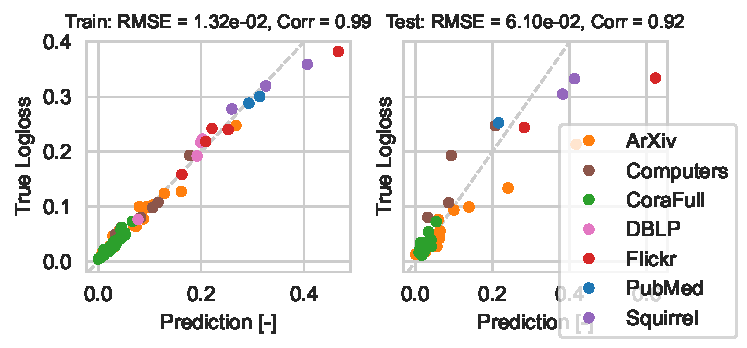
\includegraphics{images/gnn_random_split_prec_logloss.pdf}}
\end{frame}

\begin{frame}
	\frametitle{Interpretation -- Impact on Log Loss}
	\scalebox{1} {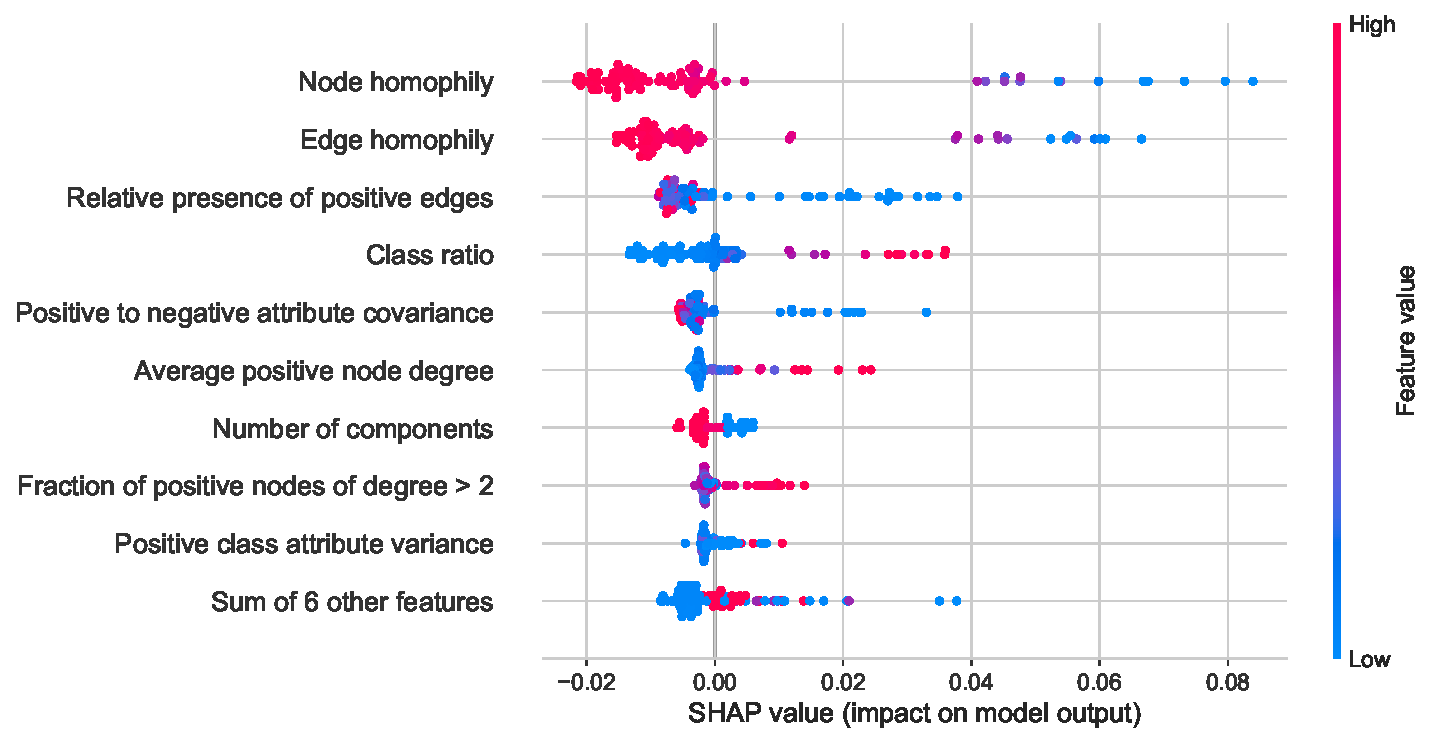
\includegraphics[width=0.9\linewidth]{images/shap_logloss.pdf}}
\end{frame}

\begin{frame}
	\frametitle{Hyper-Parameter Tuning Experiment Setup}
	\begin{itemize}
    \item Goal -- select hyper-parameter setup of GNN for a given task
    \item Evaluation -- obtained mean true GNN performance based on training set size
    \item Procedure -- fit again the regression model on training set and predict the performance on test set
\end{itemize}
\begin{columns}
\begin{column}{0.4\linewidth} 
\scalebox{0.4}{
\begin{tikzpicture}[scale=0.7]
\def\dist{1.5cm}
\tikzset{node distance=\dist, minimum size=1ex}
	\tikzset{classA/.style={circle, draw=black, fill=blue!20!yellow}}
	\tikzset{classB/.style={circle, draw=black, fill=blue!20}}
	\tikzset{classC/.style={circle, draw=black, fill=yellow!20!red}}
	\tikzset{class1/.style={circle, draw=black, fill=red!50}}
	\tikzset{class0/.style={circle, draw=black, fill=white}}
	\tikzset{desc/.style={rectangle, anchor=west, text width=2.5cm,minimum height=1cm,minimum width=2.8cm, rounded corners=1ex, align=center}}

	\newcommand{\drawgraph}[9]{
\begin{scope}[xshift=#1, yshift=#2]
\node[#3] (#9A1) {};
\node[#4, right of=#9A1] (#9A2) {};
\node[#5, below of=#9A1] (#9B1) {};
\node[#6, right of=#9A2] (#9B2) {};
\node[#7, below of=#9A2] (#9C1) {};
\node[#8, below of=#9B2] (#9C2) {};
\draw [-] (#9A1) -- (#9A2);
\draw [-] (#9A1) -- (#9B1);
\draw [-] (#9B1) -- (#9C1);
\draw [-] (#9C1) -- (#9B2);
\draw [-] (#9B2) -- (#9C2);
\draw [-] (#9A2) -- (#9B2);
\end{scope}
	}

\drawgraph{0cm}{0cm}{classA}{classA}{classB}{classB}{classC}{classC}{base}
\drawgraph{6cm}{3cm}{class1}{class1}{class0}{class0}{class0}{class0}{task1}
\drawgraph{6cm}{0cm}{class0}{class0}{class1}{class1}{class0}{class0}{task2}
\drawgraph{6cm}{-3cm}{class0}{class0}{class0}{class0}{class1}{class1}{task3}
\drawgraph{13cm}{6.2cm}{class1}{class1}{class0}{class0}{class0}{class0}{task1par1}
\drawgraph{13cm}{3cm}{class1}{class1}{class0}{class0}{class0}{class0}{task1par2}
\drawgraph{13cm}{-3cm}{class0}{class0}{class0}{class0}{class1}{class1}{task3parN}
\draw[->, thick, shorten >=1ex, shorten <=1ex] (baseB2) -- (task1B1) node [pos=0.5, above, sloped] {\small{task 1}};
\draw[->, thick, shorten >=1ex, shorten <=1ex] ([yshift=-0.5cm] baseB2.east) -- ([yshift=-0.5cm] task2A1.west) node [pos=0.5, above, sloped] {\small{task 2}};
\draw[->, thick, shorten >=1ex, shorten <=1ex] (baseC2) -- (task3A1) node [pos=0.5, above, sloped] {\small{task 3}};
\draw[->, thick, shorten >=2ex, shorten <=1ex] (task1B2) -- ([yshift=2ex] task1par1B1.west) node [pos=0.5, above, sloped] {\small{setup 1}};
\draw[->, thick, shorten >=1ex, shorten <=1ex] ([yshift=-0.5cm] task1B2.east) -- ([yshift=-0.5cm] task1par2A1.west) node [pos=0.5, above, sloped] {\small{setup 2}};
\draw[->, thick, shorten >=2ex, shorten <=1ex] ([yshift=-0.5cm] task3B2.east) -- ([yshift=-0.5cm] task3parNA1.west) node [pos=0.5, above, sloped] {\small{setup M}};

\draw[dotted, line width=3pt, shorten >=5ex, shorten <=5ex] (task1par2C1) -- (task3parNA2);

\end{tikzpicture}}
    \end{column}

    \begin{column}{0.6\linewidth}
           \scalebox{0.55}{
    \begin{tabular}{p{2cm}p{4.3cm}p{5cm}}
        \toprule
        Method Name  & required GNN runs &  Procedure Description \\
        \midrule
        Optimal & All data-points & The best setup for given  task over all setups. \\ 
        Best Hyper-Parameter & All data-points & The setup with the best average performance over tasks for given data set. \\    
        Reference & Train set & Setup with the true best performance on training set + 1 random sample on testing set.\\
        Ours & Train set &  As reference with the best predicted performance on testing set instead of the random one.\\
        Ours -- cross-datasets & Train set + data-points from all datasets excepting the investigated one &  As in ours, but the model is trained also on other datasets.\\
        \bottomrule
    \end{tabular}
    } 
    \end{column}


\end{columns}

\end{frame}

\begin{frame}
	\frametitle{Hyper-Parameter Tuning Results}
	\scalebox{1} {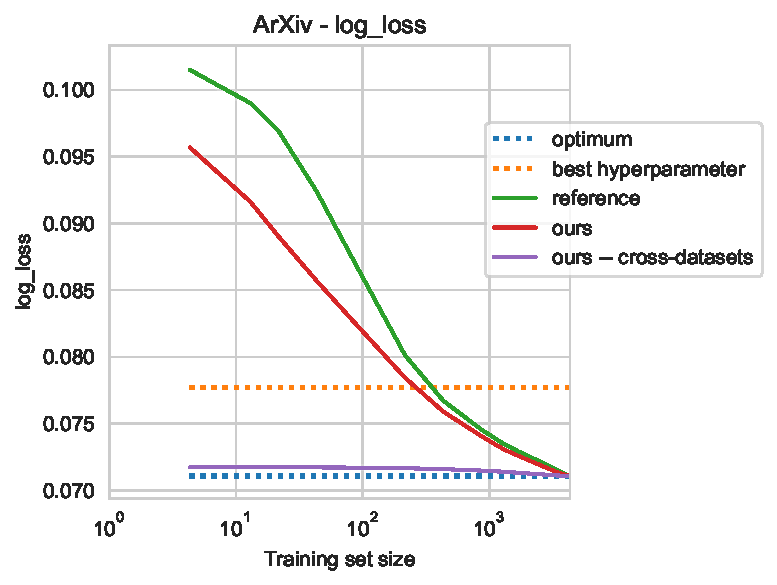
\includegraphics[width=0.7\linewidth]{images/hyperpar_tuning_small_single.pdf}}
\end{frame}

\begin{frame}
	\frametitle{Hyper-Parameter Tuning Results}
	\scalebox{1} {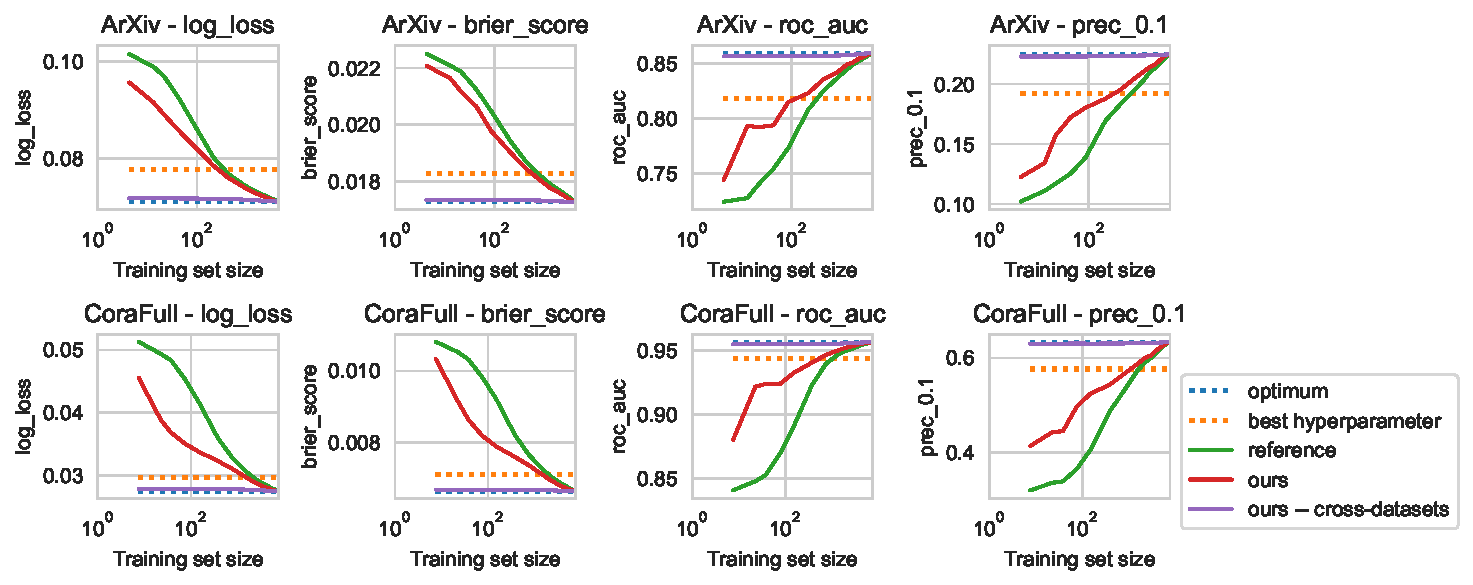
\includegraphics[width=0.9\linewidth]{images/hyperpar_tuning_small1.pdf}}
\end{frame}

\begin{frame}
	\frametitle{Hyper-Parameter Tuning Results}
	\scalebox{1} {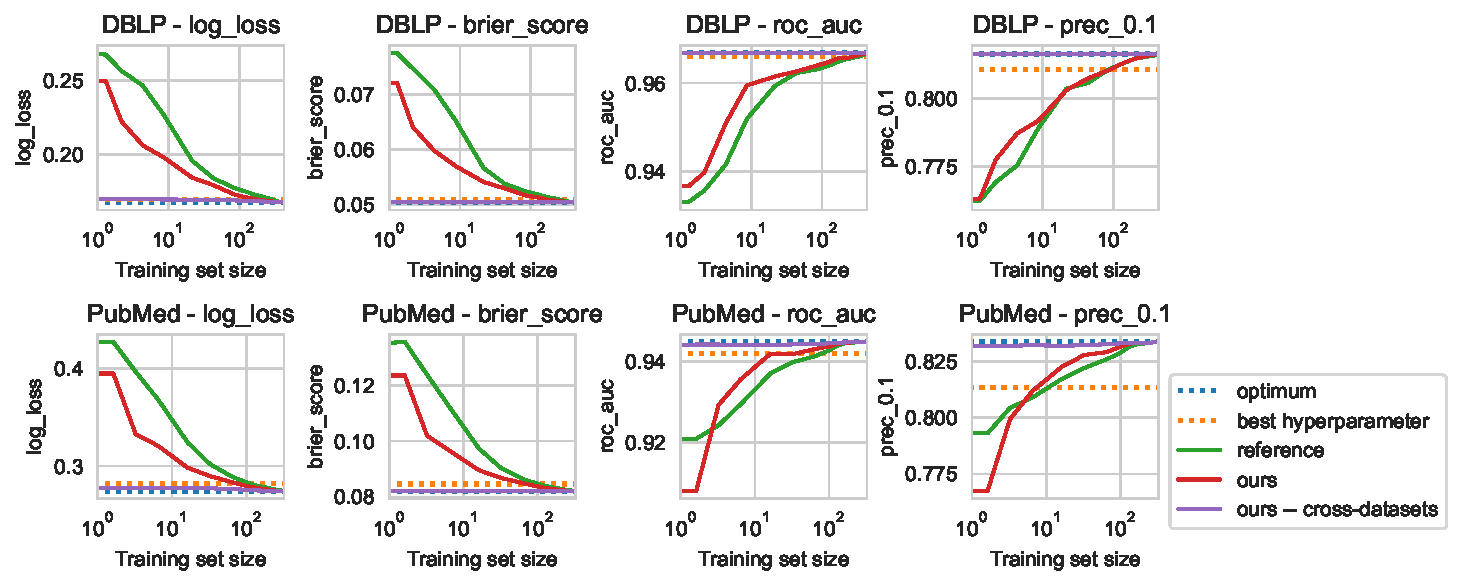
\includegraphics[width=0.9\linewidth]{images/hyperpar_tuning_small2.pdf}}
\end{frame}

\begin{frame}
	\frametitle{Hyper-Parameter Tuning Results}
	\scalebox{1} {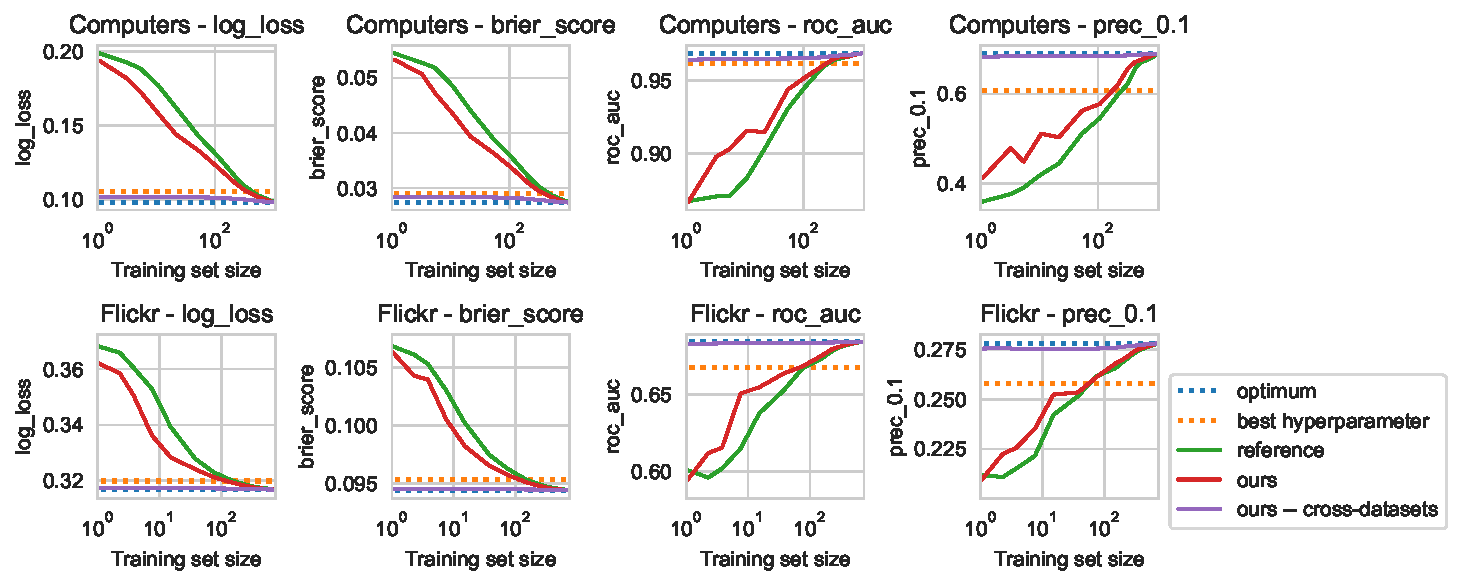
\includegraphics[width=0.9\linewidth]{images/hyperpar_tuning_small3.pdf}}
\end{frame}

\begin{frame}
	\frametitle{Conclusions}
	\begin{itemize}
		\item Proposed a method for identification of important graph
dataset properties using meta-model
		\item Hyper-parameter tuning method
based on the meta-model
		\item Experimental validation of meta-model generalization capability
		\item Evaluated importance of graph properties and their impact on GNN performance
		\item Very promissing results of hyper-parameter search method
		\item More details can be found in the paper: \cite{prochazka_which_2023}
	\end{itemize}
\end{frame}

\begin{frame}{Bibliography}
	\printbibliography
\end{frame}

\begin{frame}
	\titlepage
\end{frame}

\end{document}
